
%%%
%%% CHAPTER
%%%
\chapter{First Law of Thermodynamics}\label{Chapter:FirstLaw}

   \begin{LearningObjectivesBlock}{Learning Objectives}
      Upon completion of this chapter, you will be able to
        \begin{enumerate}
           \item Demonstrate understanding of key concepts of energy and the first law of thermodynamics;
           \item Apply the first law of thermodynamics to assess of heat transfer and power cycles;
           \item Conduct energy analysis of thermodynamic systems;
           \item Employ energy and mass balances into thermodynamic systems to assess efficiency, and correctly observe sign conventions for work and heat transfer.
        \end{enumerate}
\medskip
     Recommended reading: Chapters 2 of \citet{Atkins_Book,SmithVanNess_Book,Moran_Book} or 3 of \citet{Borgnakke_Book}.
   \end{LearningObjectivesBlock}

%%%%%%%%%%%%%%%%%%%%%%%%%%%%%%%%%%%%%%%%%%%%%%%%%%%%%%%%%%%%%%%%%
\begin{comment}
   \begin{LearningObjectivesBlock}{Learning Objectives}
      Upon completion of this chapter, you will be able to
        \begin{enumerate}
           \item {\bf Knowledge:} Define, Name, Select, State 
           \item {\bf Comprehension:} Describe, Identify, Discuss
           \item {\bf Application:} Apply, Demonstrate, Employ, Sketch
           \item {\bf Analysis:} Analyse, Compare, Calculate, Solve
           \item {\bf Synthesis:} Determine, Formulate
           \item {\bf Evaluation:} Assess, Check, Estimate, Compare, Measure, Monitor
        \end{enumerate}
\medskip
     Recommended reading: Chapters 2 of \citet{Atkins_Book,SmithVanNess_Book,Moran_Book} or 3 of \citet{Borgnakke_Book}.
   \end{LearningObjectivesBlock}
\end{comment}

   
%%%
%%% SECTION
%%%
     \section{Introduction}\label{Chapter:FirstLaw:Section:Intro}\index{Work}\index{Heat}\index{Energy}
     In Section~\ref{Chapter:Introduction:Section:ThermodAnalysis}, the main elements in the thermodynamic analysis were introduced, namely {\bf open, closed and isolated systems}, {\bf surroundings} and {\bf boundaries}. The concept of {\bf energy}, {\bf work} and {\bf heat}, pivotal entities in the study of thermodynamics systems, were also defined as,
     \begin{itemize}
        \item {\bf Work} is motion against an opposing force (Eqn.~\ref{Chpt01_Work1});
        \item {\bf Energy} of a system is its capacity to produce work, and; 
        \item {\bf Heat} is the transfer of energy across the boundary caused by temperature gradient \citep{Devoe_Book}.
     \end{itemize}
     These definitions are based on observations of systems in a macro-scale, and are critical for mass and energy balances necessary for this chapter. 

%%%
%%% SECTION
%%%
     \section{The Internal Energy}\label{Chapter:FirstLaw:Section:ThermalEnergy}\index{Internal Energy}\index{Energy!Internal|see{Internal Energy}}
     \begin{subequations}
        A system, with a prescribed amount of mass, contains energy in the form of {\bf internal energy} ($U$, inherent in the internal structure), kinetic energy (linked to the motion) and potential energy (associated with external forces acting upon the mass). The total energy, $E$, associated to the system can then be expressed as 
        \begin{displaymath}
            E = \text{Internal} + \text{Kinetic} + \text{Potential} = U + E_{\text{K}} + E_{\text{P}},
        \end{displaymath}
        and the specific energy, $e$, becomes
        \begin{equation}
            e = \frc{E}{m} = u + e_{\text{K}} + e_{\text{P}} = u + \frc{1}{2}v^{2} + gz,\label{Chapter:FirstLaw:Eqn:TotalEnergy1}
        \end{equation}
        where the kinetic energy\footnote{Kinetic energy has three components: vibrational (due to the energy associated with vibration of the body), rotational (associated with the rotation motion) and translational (associated with the motion from one spatial coordinate to another).} is assumed to be due to the translational motion (thus vibrational and rotational motion are neglected) and the potential energy to be due to the constant gravitational force. In Eqn.~\ref{Chapter:FirstLaw:Eqn:TotalEnergy1}, $u$, $e_{\text{K}}$ and $e_{\text{P}}$ are specific internal, kinetic and potential energies, respectively. Kinetic and potential energies are associated with the physical state and spatial coordinates of the system, and are commonly named {\it mechanical energy}\index{Energy!Mechanical}.  The internal energy is a characteristic of the thermodynamic state of the mass and is often labelled as {\it thermal energy}\index{Energy!Thermal}.
      
       \begin{shaded}
          The internal energy is a {\it state function}, \ie its value depends only on the current state of the system and is independent of processes undertook by the system. In other words, it is a function of the properties that determine the current state of the system.
       \end{shaded}

       Let's consider a {\it control volume} with a prescribed mass; an {\it energy balance} can be performed over this control volume assuming that energy can not be either created or destroyed but just transformed. Thus, any change in energy must be due to the transfer of energy into or out of the control volume, which can be represented as work ($W$) or heat ($Q$) transfers,
      \begin{equation}
        \frc{d\mfr[E]{}{\text{cv}}}{dt} = \mfr[\dot{E}]{}{\text{cv}} = \dot{Q} + \dot{W},\label{Chapter:FirstLaw:Eqn:TotalEnergy2}
      \end{equation}
      where the {\it dot} symbol $\left(\mathbf{\dot{ }}\right)$ over the variables represents the rate of change, \ie
      \begin{displaymath}
        \left[^{\mathbf{\cdot}}\right] =\frc{d\left[^{\mathbf{\cdot}}\right]}{dt}.
      \end{displaymath}
      Equation~\ref{Chapter:FirstLaw:Eqn:TotalEnergy2} represents the rate of change (\ie {\it instantaneous rate}) of the total energy stored in the control volume, where part of the system's energy can be transferred from or into the surroundings of the control volume. In most cases, we are interested in finite changes of properties from the beginning of the process to its end, rather than instantaneous rate evaluations. In such cases, we just need to integrate the energy equation (Eqn.~\ref{Chapter:FirstLaw:Eqn:TotalEnergy1}) \wrt time, \ie from time $t_{1}$ to $t_{2}$, then after multiplying it by $dt$,
      \begin{equation}
        \mfr[dE]{}{\text{cv}} = dU + dE_{\text{K}} + d E_{\text{P}} = \delta Q + \delta W,\label{Chapter:FirstLaw:Eqn:TotalEnergy3}\footnote{Here, it is important to differentiate three mathematical symbols commonly used in thermodynamics: $d$, $\partial$ and $\delta$. $d$ and $\partial$ represent {\it exact (or total)} (Appendix~\ref{Appendix_Calculus:TotalDifferential}) and {\it partial} (Appendix~\ref{Appendix_Calculus:PartialDifferential}) differentials, respectively. $\delta$ is often used in thermodynamics study to represent {\it inexact differential} for heat and work as these variables are path-dependent.}
      \end{equation}
      we can integrate it from {\it state 1} $\left(\text{\ie at time }t_{1}\right)$ to {\it state 2} as,
      \begin{displaymath}
        \text{\bf Left-hand side: } \int\limits_{\mfr[E]{1}{cv}}^{\mfr[E]{2}{cv}}d\mfr[E]{}{cv} = \mfr[E]{t_{2}}{cv} - \mfr[E]{t_{1}}{cv} = \mfr[E]{2}{cv} - \mfr[E]{1}{cv},
      \end{displaymath}
      \begin{displaymath}
        \text{\bf Right-hand side: } \int\limits_{t_{1}}^{t_{2}} \left|\dot{Q} + \dot{W}\right|dt = \int\limits_{\text{path}}\delta Q +  \int\limits_{\text{path}}\delta W = Q_{1-2} + W_{1-2},
      \end{displaymath}
      leading to
      \begin{equation}
          \mfr[E]{2}{cv} - \mfr[E]{1}{cv} = \left[U_{2}-U_{1}\right] + \left[\frc{1}{2}m\left(v_{2}^{2}-v_{1}^{2}\right)\right] + \left[m g \left(z_{2}-z_{1}\right)\right] = Q_{1-2} + W_{1-2}.\label{Chapter:FirstLaw:Eqn:TotalEnergy3}
      \end{equation}
      Equation~\ref{Chapter:FirstLaw:Eqn:TotalEnergy3} describes the energy balance of a system with the surroundings, where the state functions (here represented by the total, internal, kinetic and potential energies) are path-independent, whereas {\bf changes in heat and work depend on the path used in the process}. 
     \end{subequations}

%%%
%%% SECTION
%%%
     \section{Exact and Inexact Differentials}\label{Chapter:FirstLaw:Section:ExactInexactDiff}\index{Exact differential}
     %\begin{subequations}
         In Chapter~\ref{Chapter:Introduction}, we briefly defined {\it state functions}\index{State function} as thermodynamic properties that are independent of the process. For example, when water is boiled isobarically from 15$^{\circ}$C to 100$^{\circ}$C, there are infinite ways in which boiling can progress (\eg intense heat in the first 5 mins and a moderate one afterwards 'till boiling or continuous moderate heating, etc). The rate of change of the internal energy is calculated based {\bf only} on the initial and final states. The way in which the heating of water is conducted does not affect the calculation of $\Delta U$. Processes that describe the changes of state (\eg from state 1 at 15$^{\circ}$C to state 2 at 100$^{\circ}$C) are often called {\bf path functions}\index{Path function}. Examples of path functions are heat ($Q$) and work ($W$), whereas $U$ is a state function. 

        Figure~\ref{Chapter:FirstLaw:Fig:StateFunctions} shows three distinct processes (paths I-III) in which the internal energy dropped from $U_{1}$ to $U_{2}$ due to changes in heat and work. If the system is taken through any of these paths, the overall change from $U_{1}$ to $U_{2}$ is the sum (\ie integral) of all the infinitesimal changes along the path,
        \begin{displaymath}
             \Delta U = \int\limits_{1}^{2} dU.
        \end{displaymath}
        The value of $\Delta U$ depends on the initial (1) and final (2) states of the system but is independent of the path between them. Such path-independence of the integral is represented by $dU$ which is said to be an {\bf exact differential} (\ie an infinitesimal quantity in which the results after integration are independent of the path between states 1 and 2.)\index{Exact differential}. If the system is heated, the total energy transferred as heat is the sum (\ie integral) of all individual contributions throughout the pathway,
        \begin{displaymath}
             Q = \int\limits_{1,\text{path}}^{2}dQ.
        \end{displaymath}
        As heat is not a state function and the path affects the integration, the left-hand side is written as $Q$ rather than $\Delta Q$, \ie heat {\bf can not} be expressed as just $Q_{2}-Q_{1}$. Such path-dependent quantity is expressed by saying that $\delta Q$ is an {\bf inexact differential}\index{Inexact differential}, \ie an infinitesimal quantity in which the results after integration between initial and final states depends on the path.  In a similar way, the work done in  (or produced by) a system is also a path function and as such can be represented as either $\delta W$\footnote{In most thermodynamic text-books, exact and inexact differential operators, $d$ and $\delta$, are often used interchangeably for path-dependent quantities.}

     %\end{subequations}

% Figure
   \begin{figure}[h]
     \begin{center}
       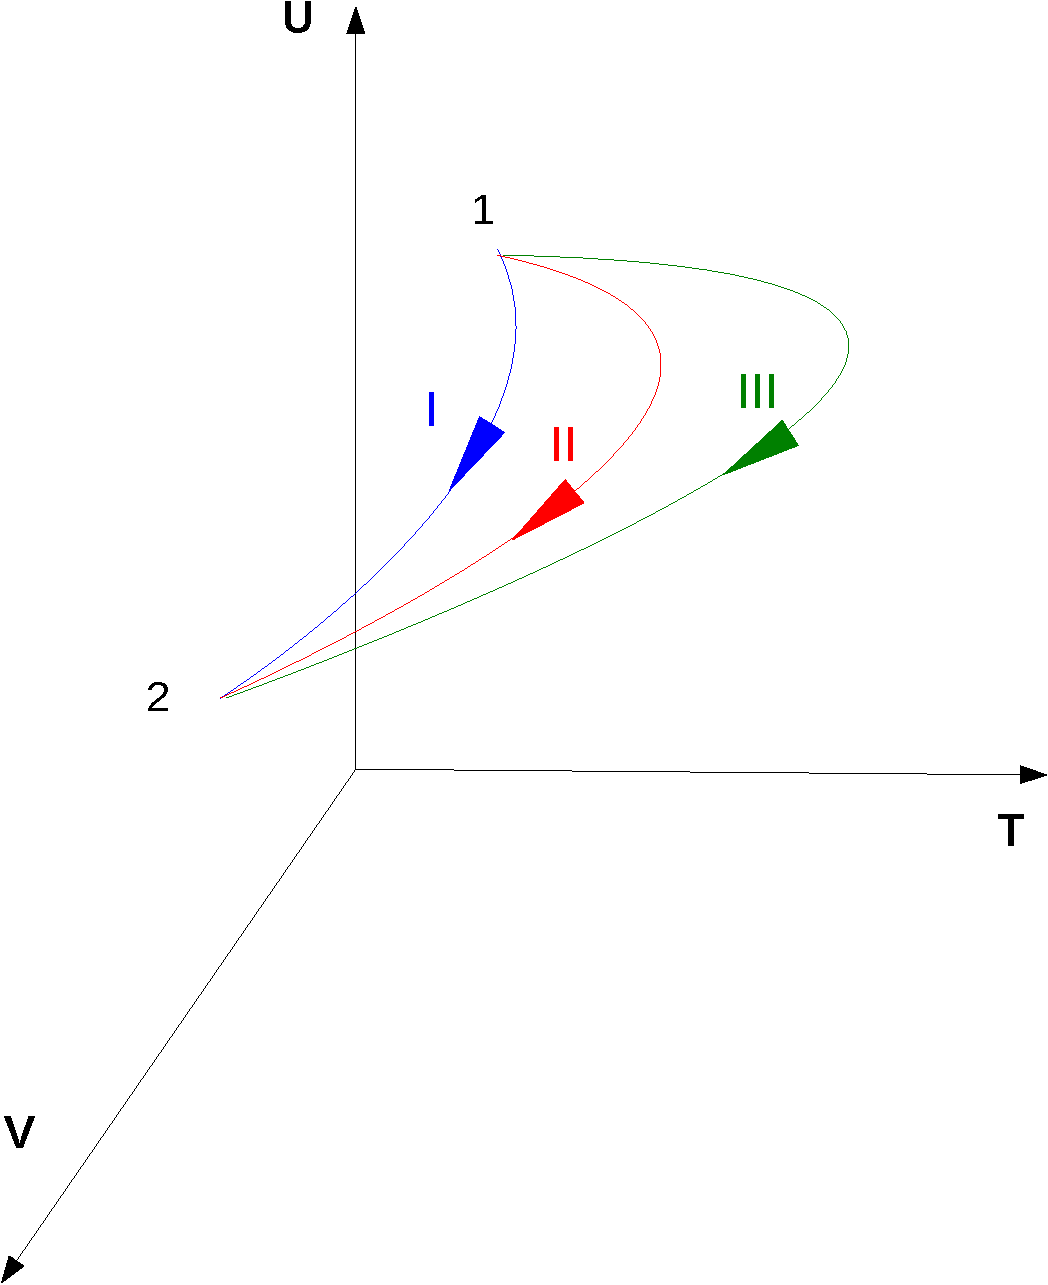
\includegraphics[width=9cm, height=9cm]{./Figs/Chp3_State-PathFunctions}
        \caption{State function: Change of internal function as a result of work and heat being exerted into the system by 3 distinct paths. Note that regardless the chosen path (from state 1 to state 2), $U_{1}$ and $U_{2}$ remain the same, although the amount of heat (represented here by changes in temperature, $T$) and work (\ie changes in volume, $V$) may vary significantly.}\label{Chapter:FirstLaw:Fig:StateFunctions}
     \end{center}
   \end{figure}


%%%
%%% SECTION
%%%
   \section{Reversible and Irreversible Processes}\label{Chapter:FirstLaw:Section:Reversibility}\index{Reversible process}\index{Irreversible process}
   Thermodynamic processes may change the state in two distinct ways:
   \begin{itemize}
     \item {\bf Reversible process} (also known as quasi-static process) is a process which can be stopped at any stage and reversed so that the system and the surroundings are exactly restored to their original states;
     \item {\bf Irreversible process} is a process in which heat is transferred through a finite temperature, thus it is not possible to return both the system and the surroundings to their original states.
   \end{itemize}
   Irreversibilities are of two types:
   \begin{itemize}
      \item {\it external irreversibilities} which are associated with dissipating effects outside the working fluid, \eg mechanical friction during a process due to some external force;
      \item {\it internal irreversibilities} which are associated with dissipating effects within the working fluid, \eg viscosity and inertial of a gas.
   \end{itemize}
   A set of definitions, characteristics and examples of these two processes are given by Table~\ref{Chapter:FirstLaw:TableDiffRevIrrev}. 
   
   
%%%
%%% SECTION
%%%
     \section{The First Law of Thermodynamics}\label{Chapter:FirstLaw:Section:FirstLaw}\index{Laws of Thermodynamics ! First law}
     \begin{subequations}
         Thermal energy is a macro-scale representation of micro-scale changes in mechanical energy (\ie work and heat). In a molecular scale, atoms and molecules are in random motion that can be associated with the kinetic energy of these `particles'. Tracking the motion and energy of each particle is addressed by a field of science called statistical (or quantum) thermodynamics; here we are interested in the consequences of the particles' motion, \ie oscillations in temperature as a measure of the average molecular-scale kinetic energy.

         \begin{shaded}
            \begin{center} {\bf Sign Notation}\end{center} 
              Before we proceed stating the {\it First Law}, we should define a sign notation used for all quantities in this document. Thus any form of energy:
              \begin{itemize}
                  \item Added to the system is assumed \blue{positive}, and;
                  \item Removed from the system is assumed \red{negative}.
              \end{itemize}
              Hence:
              \begin{itemize}
                 \renewcommand{\labelitemi}{$\star$}
                 \item heat added to the system by the neighbourhood is \blue{positive};
                 \item heat removed from the system to the neighbourhood is \red{negative};
                 \item work produced by the system and transferred to the neighbourhood is \red{negative};
                 \item work produced by the neighbourhood and transferred to the system is \blue{positive}.
              \end{itemize}
         \end{shaded}

   %%%
   %%%
   \begin{landscape}
     \begin{table}
       \begin{tabular}{||l | l||}
         \hline\hline
             {\bf Reversible process} (RP)                                    &         {\bf Irreversible process}  (IP)                          \\
         \hline
             (a) RP can not be realised in practice;                          &  (a) All practical processes occurring are IP;                    \\
             (b) The process can be carried out in the reverse direction      &  (b) The process if carries out in reverse direction, it follows  \\
                 following the same path as followed in forward direction;    &      the path different from that in forward direction;           \\
             (c) A RP leaves no trace of occurrence of process upon the       &  (c) The evidences of process having occurred are evident even    \\
                 the system and surroundings after its reversal;              &      after reversal of IP;                                        \\
             (d) Such processes can occur in either directions without        &  (d) Occurrence of IPs in either directions is not possible, as   \\
                 violating the Second Law of Thermodynamics;                  &      in one direction it shall be accompanied with the violation  \\
                                                                              &      of the Second Law of Thermodynamics;                         \\
             (e) A system undergoing RPs has maximum efficiency. Therefore,   &  (e) Systems undergoing IPs do not have maximum efficiency as it  \\
                 sytems with RPs are considered as reference systems (\ie     &      accompanied by waste of energy;                              \\
                 benchmarks);                                                 &                                                                   \\
             (f) RPs occur at infinitesimal rate, \ie quasi-static process;   &  (f) IP occur at finite rate;                                     \\
             (g) System remains in thermodynamic equilibrium during occurrence&  (g) Systems does not remain in thermodynamic equilibrium during  \\
                 of such processes;                                           &      IPs;                                                         \\
         \hline
                                 {\bf Examples}                               &             {\bf Examples}                                        \\
             (h) Frictionless motion, controlled expansion and compression,   &   (h) Viscous fluid flow, inelastic deformation and hysteresis    \\
                 elastic deformations, polytropic expansion and compression   &       effects, free expansion, throttling processes, heat transfer\\
                 of fluids, electrolysis etc.                                 &       combustion, free expansion, diffusion etc.                  \\
         \hline\hline
       \end{tabular}
       \caption{Differences between reversible and irreversible processes \citep[extracted from][]{Singh_Book}.}
       \label{Chapter:FirstLaw:TableDiffRevIrrev}
     \end{table}
   \end{landscape}
   

         In most thermodynamic systems, changes in kinetic and potential energies are often assumed negligible\footnote{Here, we are assuming that such systems are not movable \wrt frames of reference.}, and Eqn.~\ref{Chapter:FirstLaw:Eqn:TotalEnergy3} becomes
            \begin{equation}
               \mfr[E]{2}{cv} - \mfr[E]{1}{cv} = U_{2}-U_{1} = Q_{1-2} + W_{1-2},\label{Chapter:FirstLaw:Eqn:FirstLaw1}
            \end{equation}
         in such cases, the internal energy of a system may be changed in any of the following ways: producing or receiving work and/or have heat being removed or added to the system. Heat and work are equivalent ways of changing the system's internal energy. It was experimentally observed that in isolated systems there is {\bf no} change in the internal energy.

         \begin{shaded}
            The {\it First Law of Thermodynamics} is effectively a statement of energy conservation: `the only way the energy of a closed system can be changed are through transfer of energy by work or heat' \citep{Moran_Book}. In other words: `the internal energy of an isolated system is constant' \citep{Atkins_Book}. Mathematically, these statements can be readily represented in differential form (\ie during infinitesimal changes in the state of the system) by,
            \begin{equation}
               d U = \delta Q + \delta W,\label{Chapter:FirstLaw:Eqn:FirstLaw2}
            \end{equation}
            
         \end{shaded}
   
   % Example
   \begin{MyExample}{\begin{center}{\bf Example}\end{center}}
     \begin{example}\label{Chapter:FirstLaw:Example1}\citep{Atkins_Book}
        In a power station, the water pump is located in an isolated room. The electric motor of this pump produces 15 kJ of energy as mechanical work and loose 2 kJ of heat to the surroundings. Calculate the change in internal energy of the motor.  

       {\it Here, the system is the electrical motor whereas the surroundings is the room. The work produced by the motor is $\delta W= -15$ kJ and the heat transferred from the engine to the room is $\delta Q = -2$ kJ, therefore }
          \begin{eqnarray}
             dU = \Delta U &=&  \delta Q + \delta W \nonumber \\
                &=& -15 -2 = -17\text{ kJ} \nonumber
          \end{eqnarray}
     \end{example}
   \end{MyExample}

     \end{subequations}


%%%
%%% SECTION
%%%
     \section{Work Done at Moving Boundary}\label{Chapter:FirstLaw:Section:Work}
     \begin{subequations}
        In Section~\ref{Chapter:Introduction:Section:ThermodynamicWorkHeat}, the work produced by (or exerted on) the system was defined by Eqn.~\ref{Chpt01_Work2},
           \begin{equation}
              dW = -PdV \;\;\Longrightarrow \;\; W = - \int\limits_{V_{1}}^{V_{2}} PdV,\label{Chapter:FirstLaw:Eqn:Work1}
           \end{equation}
        where $P$ is the pressure and $V$ is the variable volume. Let's consider a system comprising a cylinder containing a compressible gas $\left(\text{with }V_{1}\text{ and } P_{g} = P_{1}\right)$ with a movable piston (Fig.~\ref{Chapter:FirstLaw:Fig:Work1}). An external pressure $\left(P_{\text{ext}} > P_{1}\right)$ is imposed on the piston and continuously compress the gas until the pressures are equalised $\left(P_{\text{ext}} = P_{g} = P_{2}\right)$. At the end of such compression (\ie at state 2) $V_{2}<V_{1}$ and the work $W$ is positive, \ie energy is transferred to the system through the application of an external force. Now, let's assume that at state 2, $P_{\text{ext}}$ is replaced by a new pressure, $P^{\star}_{\text{ext}}=P_{1}$, such that $P^{\star}_{\text{ext}} < P_{\text{ext}} \left(= P_{g} = P_{2}\right)$. As the new pressure is smaller than the pressure inside the cylinder $\left(P_{2}\right)$, the gas will expand until the external and internal pressure are equal, \ie $P_{g} = P^{\star}_{\text{ext}} = P_{1}$. At the end of such expansion from $V_{2}$ to $V_{1}$, the work
           \begin{displaymath}
              W = - \int\limits_{V_{2}}^{V_{1}} PdV,
           \end{displaymath}
           is negative, \ie energy is transferred from the system to the neighbourhood. In these expansion and compression processes, two scenarios may occur: constant or variable pressures. Equation~\ref{Chapter:FirstLaw:Eqn:Work1} is solved according with these scenarios.
\medskip
% Figure
   \begin{figure}[h]
     \begin{center}
        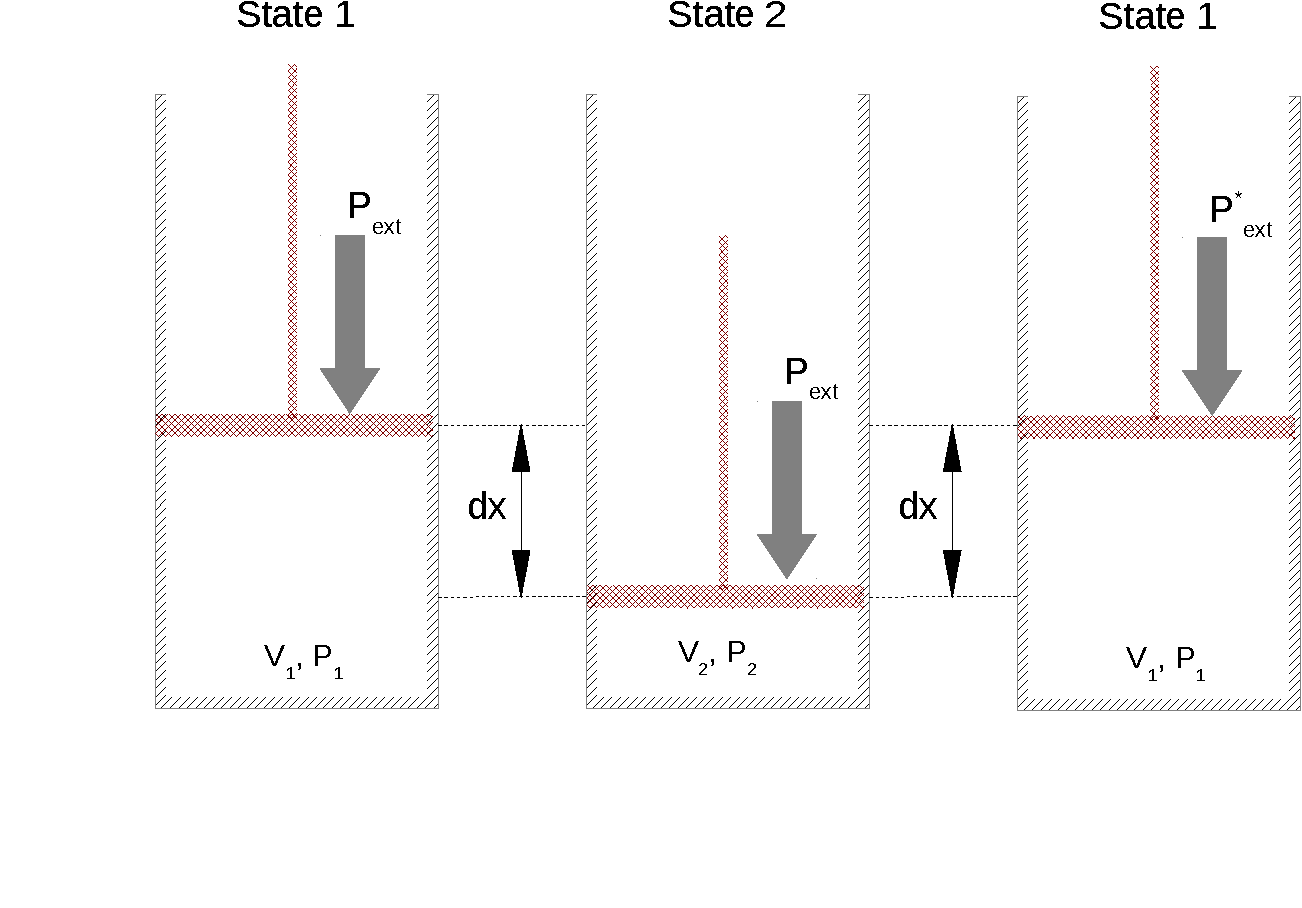
\includegraphics[width=0.7\columnwidth,clip]{./Figs/Chp3_PistonCylinder1}\vspace{-2cm}
        \caption{Compression and expansion of a piston as a result of an external force.}\label{Chapter:FirstLaw:Fig:Work1}
     \end{center}
   \end{figure}
\medskip


%%%
%%% SECTION
%%%
     \subsection{Expansion/Compression under Constant Pressure}\label{Chapter:FirstLaw:Section:Work_ConstantPressure}
        If the external pressure $P=P_{\text{ext}}$ is constant, the integral (Eqn.~\ref{Chapter:FirstLaw:Eqn:Work1}) can be readily solved with the initial and final volumes,
           \begin{shaded}
             \begin{equation}
                dW = -PdV \;\;\Longrightarrow \;\; W = - P\int\limits_{V_{1}}^{V_{2}} dV = - P\left(V_{2}-V_{1}\right) = -P\Delta V.\label{Chapter:FirstLaw:Eqn:Work_ConstPressure}
             \end{equation}
           \end{shaded}
           This integral can be graphically illustrated by the area under the $PV$ curve of Fig.~\ref{Chapter:FirstLaw:Fig:Work2}a. The work is equal to area beneath the horizontal line at $P=P_{\text{ext}}$ lying between $V_{1}$ and $V_{2}$.
           
% Figure
\begin{figure}[h]
  \vbox{
     \hbox{\hspace{2cm}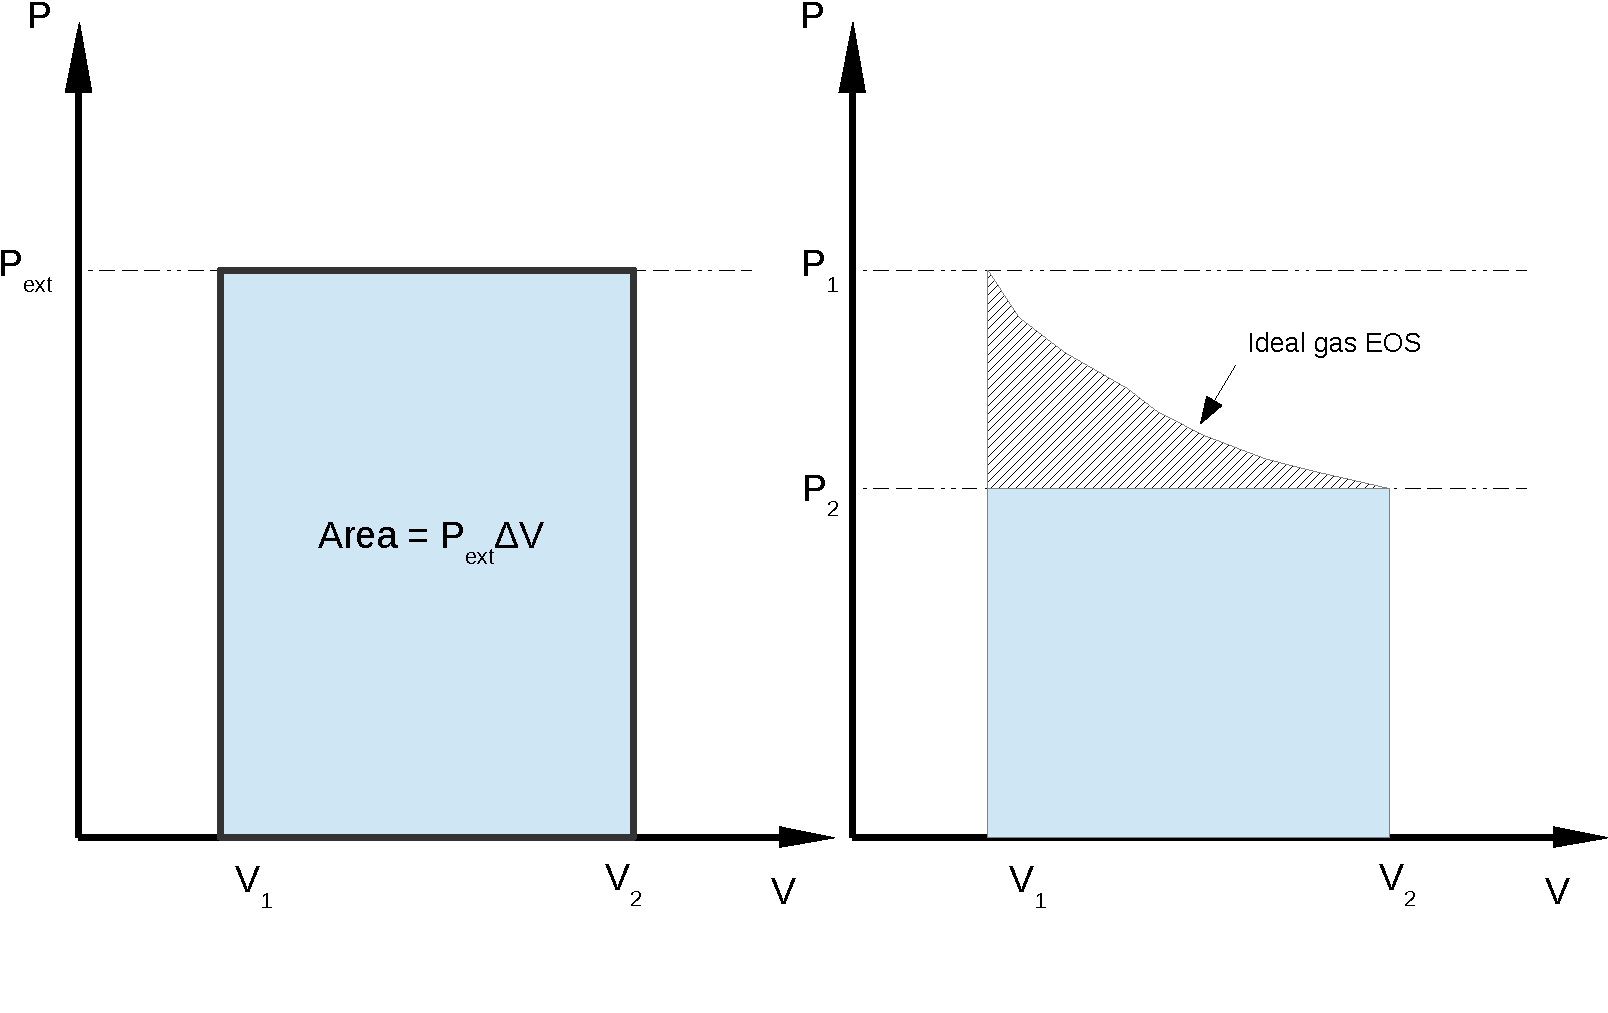
\includegraphics[width=0.7\columnwidth,clip]{./Figs/Chp3_PistonCylinder2}}
     \vspace{-1.cm}
     \hbox{\hspace{5cm}(a)\hspace{4.5cm}(b)}}%\vspace{-0.cm}
        \caption{Ideal gas expansion under isothermal conditions: (a) irreversible work at constant external pressure is equal to the blue area (Eqn.~\ref{Chapter:FirstLaw:Eqn:Work_ConstPressure}); (b) reversible work from $V_{1}$ to $V_{2}$ is given by the are below the curve (\ie blue and hatched area).}\label{Chapter:FirstLaw:Fig:Work2}
   \end{figure}

%%%
%%% SECTION
%%%
     \subsection{Reversible Expansion}\label{Chapter:FirstLaw:Section:Work_ReversibleExpansion}
     In reversible processes, changes in the state can be reversed by infinitesimal modification of a variable

A reversible change in thermodynamics is a change that can be reversed by an
infinitesimal modification of a variable. The key word ‘infinitesimal’ sharpens the
everyday meaning of the word ‘reversible’ as something that can change direction. We
say that a system is in equilibrium with its surroundings if an infinitesimal change
in the conditions in opposite directions results in opposite changes in its state. One
example of reversibility that we have encountered already is the thermal equilibrium
of two systems with the same temperature. The transfer of energy as heat between the
two is reversible because, if the temperature of either system is lowered infinitesim-
ally, then energy flows into the system with the lower temperature. If the temperature
of either system at thermal equilibrium is raised infinitesimally, then energy flows out
of the hotter system.




     
     \end{subequations}

